\documentclass[a4paper,14pt]{extarticle}

\usepackage[utf8x]{inputenc}
\usepackage[T1,T2A]{fontenc}
\usepackage[russian]{babel}
\usepackage{hyperref}
\usepackage{indentfirst}
\usepackage{here}
\usepackage{array}
\usepackage{graphicx}
\usepackage{caption}
\usepackage{subcaption}
\usepackage{chngcntr}
\usepackage{amsmath}
\usepackage{pgfplots}
\usepackage{pgfplotstable}
\usepackage[left=2cm,right=2cm,top=2cm,bottom=2cm,bindingoffset=0cm]{geometry}

\counterwithin{figure}{section}
\counterwithin{equation}{section}
\counterwithin{table}{section}
\newcommand{\sign}[1][5cm]{\makebox[#1]{\hrulefill}} % Поля подписи и даты
\graphicspath{{pics/}} % Путь до папки с картинками

\begin{document}

\begin{titlepage}
\begin{center}
	\textbf{Санкт-Петербургский Политехнический Университет \\Петра Великого}\\[0.3cm]
	\small Институт компьютерных наук и технологий \\[0.3cm]
	\small Кафедра компьютерных систем и программных технологий\\[4cm]
	
	\textbf{ОТЧЕТ}\\ \textbf{о лабораторной работе}\\[0.5cm]
	\textbf{<<Силовые преобразователи переменного напряжения в постоянное>>}\\[0.1cm]
	\textbf{Электротехника и Электроника}\\[10.5cm]
\end{center}

\begin{flushright}
	\begin{minipage}{0.60\textwidth}
		\begin{flushleft}
			\small \textbf{Работу выполнили студенты}\\[3mm]
			\small группа 23501/4 \hspace*{17mm} Дьячков В.В.\\[3mm]
			\small группа 23501/4 \hspace*{17mm} Ламтев А.Ю.\\[5mm]
			
			\small \textbf{Преподаватель}\\[5mm]
		 	\small \sign[3.5cm] \hspace*{8mm} к.т.н., доц. Кочетков Ю.Д.\\[0.5cm]
		\end{flushleft}
	\end{minipage}
\end{flushright}

\vfill

\begin{center}
	\small Санкт-Петербург\\
	\small \the\year
\end{center}
\end{titlepage}

\section{Цель работы}

Рассчитать и исследовать экспериментально различные схемы выпрямителей на полупроводниковых диодах и сглаживающих фильтров.

\section{Чертеж схемы исследуемого устройства}

\begin{figure}[h]
\begin{center}
	\begin{subfigure}[b]{0.35\textwidth}
		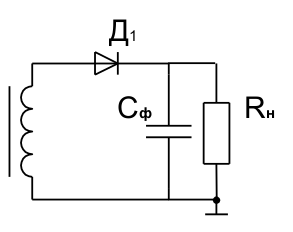
\includegraphics[scale=0.75]{diod}
		\caption{Однополупериодный \\выпрямитель}
	\end{subfigure}
	\begin{subfigure}[b]{0.35\textwidth}
		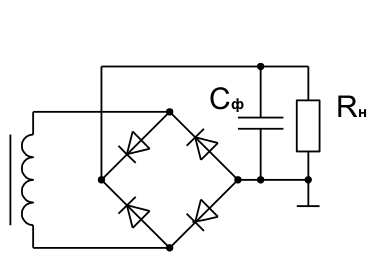
\includegraphics[scale=0.40]{four-diods}
		\caption{Двухполупериодный \\мостовой выпрямитель}
	\end{subfigure}
	\caption{}
\end{center}
\end{figure}

\vspace{-1cm}

\begin{figure}[H]
\begin{center}
	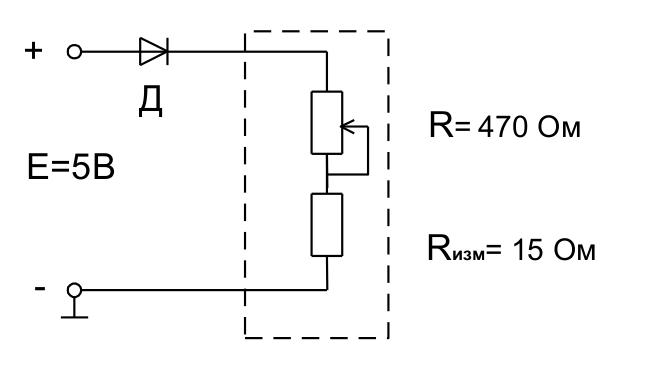
\includegraphics[width=7cm]{vac}
	\caption{Цепь для снятия вольт-амперной характеристики}
\end{center}
\end{figure}

\section{Исходные данные}

\begin{table}[H]
\begin{center}
	\caption{Исходные данные}
	\def\arraystretch{1.3}
	\def\tabcolsep{20pt}
	\begin{tabular}{|c|c|c|c|c|c|}
		\hline
		$I_\text{н ном}$, мА & $R_\text{изм}$, Ом & $R_\text{н}$, Ом & $C_\text{ф}$, мкФ & Диод\\ 
		\hline
		120 & 15 & 470 & 1500 & 2Д212А \\
		\hline	
	\end{tabular}
\end{center}
\end{table}

\section{Теоретические расчёты}

Напряжения нагрузки для обеих схем были рассчитаны по формуле:
\begin{equation}\label{eq:u_nagr}
U_\text{н} = U_2 \cdot \sqrt{2}
\end{equation}

Теоретические зависимости пульсации напряжения от силы тока нагрузки для обоих выпрямителей были рассчитаны по формуле:
\begin{equation}\label{eq:u_puls}
U_\text{п max} = \frac{I_\text{н} \cdot \Delta t}{C\text{ф}}
\end{equation}

\subsection{Однополупериодный выпрямитель}

\[
U_\text{н} = U_2 \cdot \sqrt{2} = 6.3 \cdot 1.4 = 8.91 B
\]

\[
U_\text{п max} = \frac{I_\text{н} \cdot \Delta t}{C\text{ф}} = \frac{120 \cdot 10^{-3}\cdot 20 \cdot 10^{-3}}{1500 \cdot 10^{-6}} = 1.6 B
\]

\subsection{Двухполупериодный выпрямитель}

\[
U_\text{н} = U_2 \cdot \sqrt{2} = 6.3 \cdot 1.4 = 8.91 B
\]

\[
U_\text{п max} = \frac{I_\text{н} \cdot \Delta t}{C\text{ф}} = \frac{120 \cdot 10^{-3}\cdot 10 \cdot 10^{-3}}{1500 \cdot 10^{-6}} = 0.8 B
\]

\subsection{Аппроксимация}

Для полученной экспериментальным путем ВАХ диода была выполнена аппроксимация с использованием уравнения Эберса-Молла:
\begin{large}
\[I = I_0 (e^{\frac{U}{m \phi_t}} - 1)\]
\end{large}

% См. scripts/diod.py
Для точек 
$\{\Delta U=0.53\ \text{В}, I_\text{д}=29.3\ \text{мА}\}$ 
и 
$\{\Delta U=0.73\ \text{В}, I_\text{д}=269.3\ \text{мА}\}$ 
из набора экспериментальных данных была получена система уравнений, решением которой являются значения 
$I_0 = 7.99710 \cdot 10^{-5}$ А, $m =  3.47400$.

\newpage

\section{Экспериментально снятые зависимости}

\subsection{Полупроводниковый диод}

В таблице \ref{tab:vac} и на рисунке \ref{fig:vac} изображена вольт-амперная характеристика используемого диода.

\begin{table}[H]
\begin{center}
	\caption{ВАХ полупроводникового диода}\label{tab:vac}
	\def\arraystretch{1.3}
	\def\tabcolsep{17pt}
	\pgfplotstabletypeset[col sep=comma,
	    columns={u1,u2,u,u_izm,i},
	    column type/.add={|c|}{},
	    columns/u1/.style={fixed, precision=2, zerofill, column name={$U_1$, В}},
	    columns/u2/.style={fixed, precision=2, zerofill, column name={$U_2$, В}},
	    columns/u/.style={fixed, precision=2, zerofill, column name={$\Delta U = U_1 - U_2$, В}},
	    columns/u_izm/.style={fixed, precision=2, zerofill, column name={$U_\text{изм}$, В}},
	    columns/i/.style={fixed, precision=1, zerofill, column name={$I_\text{д}$, мА}},
	    every nth row={1}{before row=\hline},
	    every head row/.style = {before row=\hline, after row=\hline},
	    every last row/.style = {after row=\hline}
	   ]{data/vac.csv}
\end{center}
\end{table}

\begin{figure}[H]
\begin{center}
	\begin{tikzpicture}
		\begin{axis}[
			height=0.4\textheight,
			width=0.9\textwidth,
			legend pos=north west,
			xlabel={$\Delta U$, В},
			ylabel={$I_\text{д}$, мА},
			xlabel near ticks,
			ylabel near ticks,
			xmin = 0.41,
			xmax = 0.8,
			ymin = 0,
			ymax = 400,
			grid=major
		]
		\addplot table [x=u, y=i, col sep=comma] {data/vac.csv};
		\addplot table [x=u, y=i, col sep=comma, mark=none] {data/vac_theory.csv};
		\legend{Эксп. ВАХ, Teор. ВАХ}
		\end{axis}
	\end{tikzpicture}
	\captionsetup{justification=centering,margin=1cm}
	\caption{Экспериментальная ВАХ полупроводникового диода}\label{fig:vac}
\end{center}
\end{figure}

\newpage

\subsection{Однополупериодный выпрямитель}

В таблице \ref{tab:half_wave} и на рисунках \ref{fig:half_wave_p} и \ref{fig:half_wave_n} представлены эксперементально снятые зависимости пульсации напряжения и напряжения нагрузки от тока для однополупериодного выпрямителя.

\begin{table}[H]
\begin{center}
	\caption{ВАХ однополупериодного выпрямителя}\label{tab:half_wave}
	\def\arraystretch{1.3}
	\def\tabcolsep{35pt}
	\pgfplotstabletypeset[col sep=comma,
	    columns={u_i,i,u_p,u_n},
	    column type/.add={|c|}{},
	    columns/u_i/.style={fixed, precision=3, zerofill, column name={$U_\text{изм}$, В}},
	    columns/i/.style={fixed, column name={$I_\text{н}$, мА}},
	    columns/u_p/.style={fixed, precision=3, zerofill, column name={$U_\text{п}$, В}},
	    columns/u_n/.style={fixed, precision=2, zerofill, column name={$U_\text{н}$, В}},
	    every nth row={1}{before row=\hline},
	    every head row/.style = {before row=\hline, after row=\hline},
	    every last row/.style = {after row=\hline}
	   ]{data/half_wave.csv}
\end{center}
\end{table}

Найдем значение $U_\text{н}$ при $I_\text{н} = 120$ мА. Для этого построим интерполяционный полином и вычислим его значение в точке $120$:
\[
U_\text{н} = 8.504 \text{ В}
\]

Найдем значение $U_\text{п max}$ при $I_\text{н} = 120$ мА. Для этого построим интерполяционный полином и вычислим его значение в точке $120$:
\[
U_\text{п max} = 1.116 \text{ В}
\]

\begin{figure}[H]
\begin{center}
	\begin{tikzpicture}
		\begin{axis}[
			height=0.4\textheight,
			width=0.9\textwidth,
			legend pos=north west,
			xlabel={$I_\text{н}$, мА},
			ylabel={$U_\text{п}$, В},
			xlabel near ticks,
			ylabel near ticks,
			xmin = 0,
			xmax = 300,
			ymin = 0,
			ymax = 4,
			xtick={0,50,...,300},
			grid=major,
		]
		\addplot table [x=i, y=u_p, col sep=comma] {data/half_wave.csv};
		\addplot table [x=i, y=u_p, col sep=comma, mark=none] {data/half_wave_theory.csv};
		\legend{Эксп. ВАХ, Teор. ВАХ}
		\end{axis}
	\end{tikzpicture}
	\captionsetup{justification=centering,margin=1cm}
	\caption{Зависимость пульсации напряжения от тока нагрузки для однополупериодного выпрямителя}\label{fig:half_wave_p}
\end{center}
\end{figure}

\vspace{-1.3cm}

\begin{figure}[H]
\begin{center}
	\begin{tikzpicture}
		\begin{axis}[
			height=0.4\textheight,
			width=0.9\textwidth,
			legend pos=north east,
			xlabel={$I_\text{н}$, мА},
			ylabel={$U_\text{н}$, В},
			xlabel near ticks,
			ylabel near ticks,
			xmin = 0,
			xmax = 300,
			ymin = 7,
			ymax = 9.5,
			xtick={0,50,...,300},
			ytick={7,7.5,...,9.5},
			grid=major,
		]
		\addplot table [x=i, y=u_n, col sep=comma] {data/half_wave.csv};
		\addplot table [x=i, y=u_n, col sep=comma, mark=none] {data/half_wave_theory.csv};
		\legend{Эксп. ВАХ, Teор. ВАХ}
		\end{axis}
	\end{tikzpicture}
	\captionsetup{justification=centering,margin=1cm}
	\caption{Зависимость напряжения нагрузки от тока нагрузки для однополупериодного выпрямителя}\label{fig:half_wave_n}
\end{center}
\end{figure}

\subsection{Двухполупериодный выпрямитель}

В таблице \ref{tab:full_wave} и на рисунках \ref{fig:full_wave_p} и \ref{fig:full_wave_n} представлены эксперементально снятые зависимости пульсации напряжения и напряжения нагрузки от тока для двухполупериодного выпрямителя.

\begin{table}[H]
\begin{center}
	\caption{ВАХ двухполупериодного выпрямителя}\label{tab:full_wave}
	\def\arraystretch{1.3}
	\def\tabcolsep{35pt}
	\pgfplotstabletypeset[col sep=comma,
	    columns={u_i,i,u_p,u_n},
	    column type/.add={|c|}{},
	    columns/u_i/.style={fixed, precision=3, zerofill, column name={$U_\text{изм}$, В}},
	    columns/i/.style={fixed, column name={$I_\text{н}$, мА}},
	    columns/u_p/.style={fixed, precision=3, zerofill, column name={$U_\text{п}$, В}},
	    columns/u_n/.style={fixed, precision=2, zerofill, column name={$U_\text{н}$, В}},
	    every nth row={1}{before row=\hline},
	    every head row/.style = {before row=\hline, after row=\hline},
	    every last row/.style = {after row=\hline}
	   ]{data/full_wave.csv}
\end{center}
\end{table}

Найдем значение $U_\text{н}$ при $I_\text{н} = 120$ мА. Для этого построим интерполяционный полином и вычислим его значение в точке $120$:
\[
U_\text{н} = 8.501 \text{ В}
\]

Найдем значение $U_\text{п max}$ при $I_\text{н} = 120$ мА. Для этого построим интерполяционный полином и вычислим его значение в точке $120$:
\[
U_\text{п max} = 0.574 \text{ В}
\]

\begin{figure}[H]
\begin{center}
	\begin{tikzpicture}
		\begin{axis}[
			height=0.4\textheight,
			width=0.9\textwidth,
			legend pos=north west,
			xlabel={$I_\text{н}$, мА},
			ylabel={$U_\text{п}$, В},
			xlabel near ticks,
			ylabel near ticks,
			xmin = 0,
			xmax = 300,
			ymin = 0,
			ymax = 2,
			xtick={0,50,...,300},
			grid=major,
		]
		\addplot table [x=i, y=u_p, col sep=comma] {data/full_wave.csv};
		\addplot table [x=i, y=u_p, col sep=comma, mark=none] {data/full_wave_theory.csv};
		\legend{Эксп. ВАХ, Teор. ВАХ}
		\end{axis}
	\end{tikzpicture}
	\captionsetup{justification=centering,margin=1cm}
	\caption{Зависимость пульсации напряжения от тока нагрузки для двухполупериодного выпрямителя}\label{fig:full_wave_p}
\end{center}
\end{figure}

\vspace{-1.3cm}

\begin{figure}[H]
\begin{center}
	\begin{tikzpicture}
		\begin{axis}[
			height=0.4\textheight,
			width=0.9\textwidth,
			legend pos=north east,
			xlabel={$I_\text{н}$, мА},
			ylabel={$U_\text{н}$, В},
			xlabel near ticks,
			ylabel near ticks,
			xmin = 0,
			xmax = 300,
			ymin = 7,
			ymax = 9.5,
			xtick={0,50,...,300},
			ytick={7,7.5,...,9.5},
			grid=major,
		]
		\addplot table [x=i, y=u_n, col sep=comma] {data/full_wave.csv};
		\addplot table [x=i, y=u_n, col sep=comma, mark=none] {data/full_wave_theory.csv};
		\legend{Эксп. ВАХ, Teор. ВАХ}
		\end{axis}
	\end{tikzpicture}
	\captionsetup{justification=centering,margin=1cm}
	\caption{Зависимость напряжения нагрузки от тока нагрузки для двухполупериодного выпрямителя}\label{fig:full_wave_n}
\end{center}
\end{figure}

\section{Погрешности}

\subsection{Предельно допустимые погрешности}

Номинальное значение емкости конденсатора может отклоняться от реального на 20\% в меньшую сторону и на 80\% в большую. С учетом того, что пульсация напряжения обратно пропорциональна емкости конденсатора, предельно допустимая погрешность $\delta U_\text{п}$ равна 80\% при отклонении в меньшую сторону и 20\% при отклонении в большую.

\subsection{Однополупериодный выпрямитель}

\[
\delta U_\text{п max} = \frac{U_\text{п max\ \ теор} - U_\text{п max\ \ эксп}}{U_\text{п max\ \ теор}} = \frac{1.6 - 1.116}{1.6} = 0.302 = 30.2 \%
\]

\[
\delta U_\text{н} = \frac{U_\text{н\ \ теор} - U_\text{н\ \ эксп}}{U_\text{н\ \ теор}} = \frac{8.91 - 8.504}{8.91} = 0.045 = 4.5 \%
\]

\subsection{Двухполупериодный выпрямитель}

\[
\delta U_\text{п max} = \frac{U_\text{п max\ \ теор} - U_\text{п max\ \ эксп}}{U_\text{п max\ \ теор}} = \frac{0.8 - 0.574}{0.8} = 0.282 = 28.2 \%
\]

\[
\delta U_\text{н} = \frac{U_\text{н\ \ теор} - U_\text{н\ \ эксп}}{U_\text{н\ \ теор}} = \frac{8.91 - 8.501}{8.91} = 0.046 = 4.6 \%
\]

\section{Выводы}

Приведенные погрешности $U_\text{п}$ для однополупериодного и двухполупериодного выпрямителей равны 30.2\% и 28.2\% соответственно, что не превышает предельно допустимую погрешность - 80\%.

Таким образом, теоретические формулы \ref{eq:u_nagr} и \ref{eq:u_puls} являются верными.

\end{document}
